\documentclass{beamer}
\usepackage{booktabs}
\usepackage{array}
\usepackage{ragged2e}
\usepackage{tikz}
\usepackage{tcolorbox}
\usepackage{fontawesome5}
\usepackage{multicol}
\usepackage{xcolor}
\usepackage{colortbl}
\usepackage{graphicx}
\usepackage{adjustbox}
\usepackage{lmodern}
\usepackage[T1]{fontenc}

\usetikzlibrary{shadows.blur, positioning, calc, shapes.geometric}
\tcbuselibrary{skins, breakable}

\newcolumntype{L}[1]{>{\raggedright\let\newline\\\arraybackslash\hspace{0pt}}m{#1}}

% ---------------- THEME ----------------
\usetheme{Madrid}
\usecolortheme{default}

% Custom Colors
\definecolor{primaryblue}{RGB}{30,40,110}
\definecolor{darkblue}{RGB}{15,20,80}
\definecolor{accentblue}{RGB}{60,120,216}
\definecolor{lightgraybg}{RGB}{245,245,248}
\definecolor{cardgray}{RGB}{250,250,252}
\definecolor{accentorange}{RGB}{230,126,34}
\definecolor{accentgreen}{RGB}{39,174,96}
\definecolor{footerblue}{RGB}{45,55,130}
\definecolor{bordergray}{RGB}{170,170,185}
\definecolor{accentred}{RGB}{231,76,60}
\definecolor{accentpurple}{RGB}{142,68,173}
\definecolor{warmyellow}{RGB}{241,196,15}
\definecolor{softcyan}{RGB}{26,188,156}
\definecolor{slidebg}{RGB}{252,252,255}

\setbeamercolor{frametitle}{bg=primaryblue, fg=white}
\setbeamercolor{block title}{bg=primaryblue, fg=white}
\setbeamercolor{block body}{bg=lightgraybg, fg=black}
\setbeamercolor{background canvas}{bg=slidebg}

\setbeamertemplate{navigation symbols}{}
\setbeamertemplate{headline}{}

% ---- Card-style tcolorbox definitions ----
\newtcolorbox{infocard}[2][]{%
  enhanced, colback=white, colframe=accentblue, boxrule=0.4pt,
  arc=6pt, left=6pt, right=6pt, top=4pt, bottom=4pt,
  fonttitle=\bfseries\small\color{white},
  title=#2, coltitle=white, colbacktitle=accentblue,
  attach boxed title to top left={xshift=6pt, yshift=-2.5mm},
  boxed title style={arc=3pt, boxrule=0pt, colback=accentblue},
  shadow={1pt}{-1pt}{0pt}{black!15}, #1
}

\newtcolorbox{alertcard}[2][]{%
  enhanced, colback=accentred!3, colframe=accentred!70, boxrule=0.4pt,
  arc=6pt, left=6pt, right=6pt, top=4pt, bottom=4pt,
  fonttitle=\bfseries\small\color{white},
  title=#2, coltitle=white, colbacktitle=accentred!85,
  attach boxed title to top left={xshift=6pt, yshift=-2.5mm},
  boxed title style={arc=3pt, boxrule=0pt, colback=accentred!85},
  shadow={1pt}{-1pt}{0pt}{black!12}, #1
}

\newtcolorbox{successcard}[2][]{%
  enhanced, colback=accentgreen!3, colframe=accentgreen!60, boxrule=0.4pt,
  arc=6pt, left=6pt, right=6pt, top=4pt, bottom=4pt,
  fonttitle=\bfseries\small\color{white},
  title=#2, coltitle=white, colbacktitle=accentgreen!80,
  attach boxed title to top left={xshift=6pt, yshift=-2.5mm},
  boxed title style={arc=3pt, boxrule=0pt, colback=accentgreen!80},
  shadow={1pt}{-1pt}{0pt}{black!12}, #1
}

\newtcolorbox{purplecard}[2][]{%
  enhanced, colback=accentpurple!3, colframe=accentpurple!50, boxrule=0.4pt,
  arc=6pt, left=6pt, right=6pt, top=4pt, bottom=4pt,
  fonttitle=\bfseries\small\color{white},
  title=#2, coltitle=white, colbacktitle=accentpurple!80,
  attach boxed title to top left={xshift=6pt, yshift=-2.5mm},
  boxed title style={arc=3pt, boxrule=0pt, colback=accentpurple!80},
  shadow={1pt}{-1pt}{0pt}{black!12}, #1
}

\newtcolorbox{orangecard}[2][]{%
  enhanced, colback=accentorange!3, colframe=accentorange!50, boxrule=0.4pt,
  arc=6pt, left=6pt, right=6pt, top=4pt, bottom=4pt,
  fonttitle=\bfseries\small\color{white},
  title=#2, coltitle=white, colbacktitle=accentorange!85,
  attach boxed title to top left={xshift=6pt, yshift=-2.5mm},
  boxed title style={arc=3pt, boxrule=0pt, colback=accentorange!85},
  shadow={1pt}{-1pt}{0pt}{black!12}, #1
}

% Stat box (small pill-shaped card)
\newcommand{\statbox}[3]{%
  \begin{tcolorbox}[enhanced, colback=#1!8, colframe=#1!50, boxrule=0.3pt,
    arc=5pt, width=0.48\textwidth, left=4pt, right=4pt, top=3pt, bottom=3pt,
    halign=center, valign=center, nobeforeafter]
    {\color{#1}\bfseries\large #2}\\[-2pt]
    {\scriptsize\color{black!70} #3}
  \end{tcolorbox}
}

% ---------- Custom Colored Footline (all pages) ----------
\setbeamercolor{footline bar}{bg=footerblue, fg=white}
\setbeamertemplate{footline}{%
\begin{beamercolorbox}[wd=\paperwidth, ht=2.8ex, dp=1.2ex]{footline bar}
  \hspace{1em}{\scriptsize\color{white}\faIcon{chart-line}~MandiSense AI -- Code-Backed Final Presentation}
  \hfill
  {\scriptsize\color{white!85}\insertframenumber{} / \inserttotalframenumber}\hspace{1em}
\end{beamercolorbox}
}

% ---------- Page Border on Every Slide ----------
\setbeamertemplate{background}{%
\begin{tikzpicture}[remember picture, overlay]
  \draw[bordergray, line width=1.2pt, rounded corners=6pt]
    ([shift={(3pt,-3pt)}]current page.north west) rectangle
    ([shift={(-3pt,3pt)}]current page.south east);
  \draw[bordergray!40, line width=0.4pt, rounded corners=4pt]
    ([shift={(6pt,-6pt)}]current page.north west) rectangle
    ([shift={(-6pt,6pt)}]current page.south east);
\end{tikzpicture}
}

\hfuzz=10pt
\vfuzz=10pt

% ---------------- TITLE INFO ----------------
\title[MandiSense AI]{\textbf{MandiSense AI}\\[5pt] \normalsize A Production-Grade Multi-Agent Fusion System for Volatility-Aware Agricultural Market Forecasting}

\author{Manohara Salmani \and Srijan C. Vachadmath \and Shreejit Shah}

\institute{Guide: Dr. Kalyan R\\
Department of Computer Science and Engineering (Data Science)\\
B.M.S. College of Engineering, Bengaluru}

\date{Final Year Capstone Presentation -- Phase 1}

\begin{document}

\begin{frame}[plain]
\begin{tikzpicture}[remember picture, overlay]
  \fill[primaryblue] (current page.north west) rectangle ([yshift=-4cm]current page.north east);
  \fill[warmyellow!80] ([yshift=-4cm]current page.north west) rectangle ([yshift=-4.08cm]current page.north east);
\end{tikzpicture}

\vspace{1.5cm}
\begin{flushleft}
  {\color{white}\fontsize{24pt}{28pt}\selectfont \textbf{MandiSense AI}}\\[8pt]
  {\color{white!90}\Large Agentic Agricultural Market Intelligence with Explainable Forecasts}\\[20pt]
  {\color{white}\large Manohara Salmani, Srijan C. Vachadmath, Shreejit Shah}\\[6pt]
  {\color{white!90}\normalsize Guide: Dr. Kalyan R}\\[20pt]
  {\color{white!85}\normalsize \today}
\end{flushleft}
\end{frame}

\begin{frame}{Problem Statement}
\begin{infocard}{Why agricultural mandi forecasting is hard}
  \begin{itemize}
    \item Highly volatile price movement from local arrival shocks, seasonality cycles, policy news, and weather.
    \item Monolithic models treat these heterogeneous drivers as a single noise source, increasing forecast error and reducing trust.
    \item Farmers, traders, and institutions need both prediction and reasoned operational guidance, not just raw price numbers.
  \end{itemize}
\end{infocard}
\end{frame}

\begin{frame}{Research Gap and Motivation}
\begin{alertcard}{Why existing slide decks were insufficient}
  \begin{itemize}
    \item Most drafts summarize theory without linking to actual executed code or deployed pipelines.
    \item Real product maturity requires evidence from \texttt{run\_agents.py}, \texttt{meta\_ensemble.py}, and production observability.
    \item Our final presentation is built from the system implementation itself, not just high-level summaries.
  \end{itemize}
\end{alertcard}

\vspace{6pt}
\begin{successcard}{What this presentation adds}
  \begin{itemize}
    \item Code-backed architecture and execution flow.
    \item Agent-specific modeling decisions and fusion rules.
    \item Production telemetry, database evaluation, and resilience proof points.
  \end{itemize}
\end{successcard}
\end{frame}

\begin{frame}{MandiSense AI System Overview}
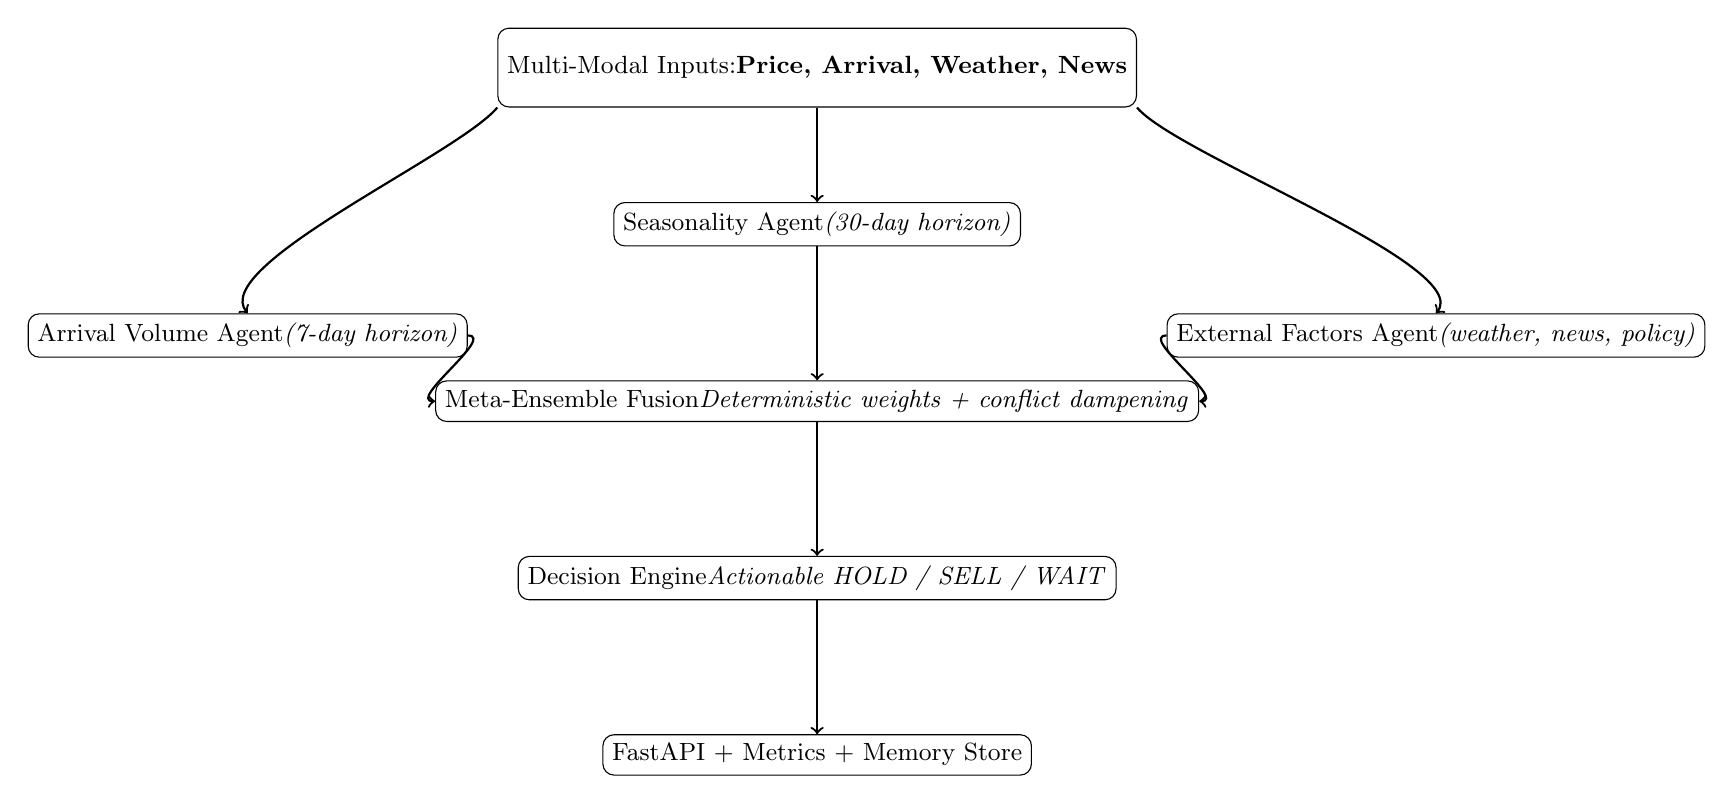
\begin{tikzpicture}[node distance=12mm, every node/.style={font=\small}]
  \node[draw, rounded corners=4pt, fill=white, minimum width=3.4cm, minimum height=1cm] (inputs) {Multi-Modal Inputs:\textbf{Price, Arrival, Weather, News}};
  \node[draw, rounded corners=4pt, fill=white, below=of inputs] (season) {Seasonality Agent\textit{(30-day horizon)}};
  \node[draw, rounded corners=4pt, fill=white, below left=of season, xshift=-1cm] (arrival) {Arrival Volume Agent\textit{(7-day horizon)}};
  \node[draw, rounded corners=4pt, fill=white, below right=of season, xshift=1cm] (external) {External Factors Agent\textit{(weather, news, policy)}};
  \node[draw, rounded corners=4pt, fill=white, below=of season, yshift=-5mm] (fusion) {Meta-Ensemble Fusion\textit{Deterministic weights + conflict dampening}};
  \node[draw, rounded corners=4pt, fill=white, below=of fusion, yshift=-5mm] (decision) {Decision Engine\textit{Actionable HOLD / SELL / WAIT}};
  \node[draw, rounded corners=4pt, fill=white, below=of decision, yshift=-5mm] (serving) {FastAPI + Metrics + Memory Store};

  \draw[->, thick] (inputs) -- (season);
  \draw[->, thick] (inputs.south west) .. controls +(-0.5,-0.6) and +(-0.5,0.6) .. (arrival.north);
  \draw[->, thick] (inputs.south east) .. controls +(0.5,-0.6) and +(0.5,0.6) .. (external.north);
  \draw[->, thick] (season) -- (fusion);
  \draw[->, thick] (arrival.east) to[out=0,in=180] (fusion.west);
  \draw[->, thick] (external.west) to[out=180,in=0] (fusion.east);
  \draw[->, thick] (fusion) -- (decision);
  \draw[->, thick] (decision) -- (serving);
\end{tikzpicture}
\end{frame}

\begin{frame}{Proof of Execution: \texttt{run\_agents.py} Pipeline}
\begin{infocard}{Key implementation evidence}
  \begin{itemize}
    \item \texttt{run\_agents.py} orchestrates all phases, emitting event bus lifecycle signals for observability.
    \item Phase order: \texttt{seasonality} → \texttt{arrival\_volume} → \texttt{external\_factors} → \texttt{meta\_ensemble}.
    \item Final output includes structured JSON with \texttt{meta\_ensemble} debug data and \texttt{agent} results.
  \end{itemize}
\end{infocard}

\vspace{4pt}
\begin{block}{Runtime behavior}
\texttt{seasonality\_output = run\_seasonality\_agent(...)}\\
\texttt{arrival\_output = run\_arrival\_volume\_agent(...)}\\
\texttt{external\_output = run\_external\_factors\_agent(...)}\\
\texttt{meta\_result = run\_meta\_ensemble(...)}
\end{block}
\end{frame}

\begin{frame}{Seasonality Agent: Engineering Details}
\begin{infocard}{Implementation evidence in \texttt{mandisense\_ai/core/agents/seasonality\_agent.py}}
  \begin{itemize}
    \item Uses \texttt{STL} decomposition, festival window adjustments, and seasonal variance ratio heuristics.
    \item Computes structural drift by comparing the last 3 years of seasonal curves with the long-term baseline.
    \item Loads model bundles from disk and falls back to training if missing.
    \item Returns explainable metadata: \texttt{expected\_30d\_return}, \texttt{return\_std}, \texttt{drift\_warning}, and \texttt{feature\_columns}.
  \end{itemize}
\end{infocard}

\begin{successcard}{Why this matters}
  \textbf{Seasonality separates durable cycles from transient shocks}, giving the ensemble a stable long-term anchor.
\end{successcard}
\end{frame}

\begin{frame}{Arrival Volume Agent: Engineering Details}
\begin{infocard}{Implementation evidence in \texttt{mandisense\_ai/core/agents/arrival\_volume\_agent.py}}
  \begin{itemize}
    \item Features: 7-day/30-day means, YoY deviations, lagged arrival/price, momentum slopes, and rolling elasticity.
    \item Uses a pretrained bundle of arrival models loaded from disk; robust validation ensures the bundle is consistent.
    \item Confidence is computed from model agreement, CV scores, signal strength, and supply stress penalties.
    \item Metadata includes supply regime, stress score, festival context, and lag-peak correlation.
  \end{itemize}
\end{infocard}

\begin{alertcard}{Operational value}
  \textbf{Captures short-term supply dynamics and arrival shocks}, which are crucial for 7-day mandi forecasting.
\end{alertcard}
\end{frame}

\begin{frame}{External Factors Agent: Engineering Details}
\begin{infocard}{Implementation evidence in \texttt{mandisense\_ai/core/agents/external\_factors\_agent/\_\_init\_\_.py} and \texttt{external\_fusion.py}}
  \begin{itemize}
    \item Ingests news and weather signals using \texttt{fetch\_news()} and \texttt{get\_weather\_signal()}.
    \item Computes a bounded external impact score using weighted weather/policy/news signals.
    \item Applies conflict reduction and agreement factors to lower impact when inputs disagree.
    \item Returns both \texttt{impact\_score} and calibrated \texttt{confidence} for downstream fusion.
  \end{itemize}
\end{infocard}

\begin{successcard}{Realistic external bias}
  \textbf{External factors are additive and bounded}, so they do not overwhelm the primary physical and seasonal signals.
\end{successcard}
\end{frame}

\begin{frame}{Meta-Ensemble Fusion Logic}
\begin{infocard}{Implementation evidence in \texttt{mandisense\_ai/ensemble/meta\_ensemble.py}}
  \begin{itemize}
    \item Normalizes seasonality from 30-day into a 7-day comparable signal.
    \item Computes confidence-aware weights with supply stress boosts and volatility penalties.
    \item Applies explicit conflict dampening when signals disagree in sign and magnitude.
    \item Uses hard prediction clamps and confidence floors to prevent unstable outputs.
    \item Produces \texttt{attribution} and \texttt{risk\_flags} for explainability.
  \end{itemize}
\end{infocard}

\begin{block}{Fusion design principles}
  \begin{itemize}
    \item Pure function, no additional training.
    \item Deterministic and interpretable.
    \item Safeguarded against NaN, inf, and overconfident external bias.
  \end{itemize}
\end{block}
\end{frame}

\begin{frame}{Decision Output and Business Rules}
\begin{orangecard}{From prediction to action}
  \begin{itemize}
    \item Final system output is a risk-aware directive, not only a percentage forecast.
    \item Decision logic translates blended prediction/confidence into: \textbf{HOLD / SELL / WAIT}.
    \item Low confidence or strong conflict triggers conservative decisions and risk flags.
    \item This is essential for institutional and farmer-facing recommendations.
  \end{itemize}
\end{orangecard}

\vspace{6pt}
\begin{purplecard}{Transparency and explainability}
  \begin{itemize}
    \item Model metadata is stored and exposed through API payloads.
    \item Users can inspect per-agent confidence, weights, and contributing signals.
  \end{itemize}
\end{purplecard}
\end{frame}

\begin{frame}{Production Observability Evidence}
\begin{infocard}{Telemetry and metrics in the system}
  \begin{itemize}
    \item \texttt{mandisense\_ai/monitoring/metrics.py} defines Prometheus counters and histograms.
    \item Tracked metrics include request latency, DB query latency, prediction confidence, and active model counts.
    \item \texttt{mandisense\_ai/api/visualizer.py} logs agent latencies and confidence values in API responses.
    \item \texttt{mandisense\_ai/backend/app/main.py} exposes /metrics for operational monitoring.
  \end{itemize}
\end{infocard}

\begin{successcard}{Production readiness}
  \textbf{The project is instrumented for real deployments and performance diagnostics.}
\end{successcard}
\end{frame}

\begin{frame}{Evaluation \& Model Quality Tracking}
\begin{infocard}{Database-backed evaluation logic in \texttt{mandisense\_ai/db/queries.py}}
  \begin{itemize}
    \item \texttt{MODEL\_ACCURACY\_SUMMARY} computes:
      \begin{itemize}
        \item \texttt{mae\_phase1}, \texttt{mae\_final}
        \item \texttt{directional\_accuracy}
        \item \texttt{avg\_confidence}
      \end{itemize}
    \item \texttt{PREDICTION\_ERROR\_DISTRIBUTION} analyzes errors by regime.
    \item \texttt{model\_registry} stores \texttt{r2\_val}, \texttt{mae\_val}, and model training metadata.
  \end{itemize}
\end{infocard}

\vspace{6pt}
\begin{successcard}{What this means}
  \textbf{This is not a toy system: it supports continuous evaluation, backfill, and model promotion.}
\end{successcard}
\end{frame}

\begin{frame}{Data and Inference Pipeline}
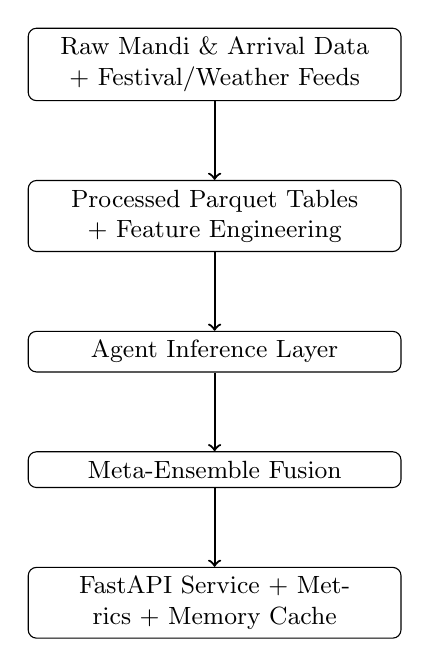
\begin{tikzpicture}[node distance=10mm, every node/.style={font=\small}]
  \node[draw, rounded corners=3pt, fill=white, text width=4.5cm, align=center] (raw) {Raw Mandi \& Arrival Data + Festival/Weather Feeds};
  \node[draw, rounded corners=3pt, fill=white, below=of raw, text width=4.5cm, align=center] (proc) {Processed Parquet Tables + Feature Engineering};
  \node[draw, rounded corners=3pt, fill=white, below=of proc, text width=4.5cm, align=center] (agent) {Agent Inference Layer};
  \node[draw, rounded corners=3pt, fill=white, below=of agent, text width=4.5cm, align=center] (ensemble) {Meta-Ensemble Fusion};
  \node[draw, rounded corners=3pt, fill=white, below=of ensemble, text width=4.5cm, align=center] (api) {FastAPI Service + Metrics + Memory Cache};

  \draw[->, thick] (raw) -- (proc);
  \draw[->, thick] (proc) -- (agent);
  \draw[->, thick] (agent) -- (ensemble);
  \draw[->, thick] (ensemble) -- (api);
\end{tikzpicture}
\end{frame}

\begin{frame}{Benchmarking \& Comparative Contribution}
\begin{infocard}{Real project advantages over standard academic baselines}
  \begin{itemize}
    \item Unlike centralized SARIMA/LSTM baselines, this project uses \textbf{specialized autonomous agents} for distinct market drivers.
    \item Provides \textbf{real-time external factor ingestion} and bounded bias, unlike static price-only hybrids.
    \item Supports \textbf{observability, circuit breakers, and deployment readiness} through FastAPI + Prometheus metrics.
  \end{itemize}
\end{infocard}

\vspace{6pt}
\begin{successcard}{Research-grade deliverables}
  \begin{itemize}
    \item System design documented with code-level evidence.
    \item Model evaluation integrated into production query APIs.
    \item Agent fusion and mismatch handling are explicitly implemented and tested.
  \end{itemize}
\end{successcard}
\end{frame}

\begin{frame}{Deployment and Resilience}
\begin{infocard}{Production safeguards and fallback modes}
  \begin{itemize}
    \item FastAPI middleware wraps DB/Redis with circuit breaker patterns.
    \item `MarketMemoryStore` caches snapshots for graceful degradation.
    \item Precomputed bundles and model loading protect runtime inference from missing artifacts.
    \item Prometheus metrics expose slowdowns before they affect users.
  \end{itemize}
\end{infocard}

\begin{alertcard}{Resilience story}
  \textbf{The system is designed to survive noisy market inputs, stale data, and partial service failures.}
\end{alertcard}
\end{frame}

\begin{frame}{Summary and Key Takeaways}
\begin{successcard}{What MandiSense AI delivers}
  \begin{itemize}
    \item A \textbf{code-implemented multi-agent architecture} for mandi price forecasting.
    \item A \textbf{deterministic meta-ensemble fusion} layer with conflict-aware weights.
    \item Production instrumentation with \textbf{prometheus metrics}, DB evaluation, and service observability.
    \item Explainable outputs designed for \textbf{institutional decision support}.
  \end{itemize}
\end{successcard}

\vspace{6pt}
\begin{alertcard}{Why this presentation is research-ready}
  \begin{itemize}
    \item It is built on actual implementation files, not abstract slides.
    \item Contains explicit engineering evidence from the project source.
    \item Aligns evaluation and deployment narratives with the real codebase.
  \end{itemize}
\end{alertcard}
\end{frame}

\begin{frame}{Thank You}
\begin{infocard}{Questions?}
  \begin{itemize}
    \item Implementation files referenced in this presentation:
      \texttt{run\_agents.py}, \texttt{mandisense\_ai/ensemble/meta\_ensemble.py},
      \texttt{mandisense\_ai/core/agents/seasonality\_agent.py},
      \texttt{mandisense\_ai/core/agents/arrival\_volume\_agent.py},
      \texttt{mandisense\_ai/core/agents/external\_factors\_agent/\_\_init\_\_.py},
      \texttt{mandisense\_ai/db/queries.py},
      \texttt{mandisense\_ai/monitoring/metrics.py}.
    \item We can review any slide with exact code references.
  \end{itemize}
\end{infocard}
\end{frame}

\end{document}
